\documentclass[10pt]{article}
\usepackage{../NotesTeX}

\newcommand{\diff}{\mathrm{d}}
\newcommand{\dom}{\mathrm{dom}}
\newcommand{\cod}{\mathrm{cod}}
\newcommand{\im}{\mathrm{im}}
\newcommand{\N}{\mathbb{N}}
\newcommand{\Z}{\mathbb{Z}}
\newcommand{\Q}{\mathbb{Q}}
\newcommand{\R}{\mathbb{R}}

\graphicspath{ {../img} }

\title{Lorem Ipsum}

\author{Marcos Ávila Navas}
\affiliation{I.E.S Los Colegiales}

\begin{document}

\maketitle

\flushbottom
\newpage
\pagestyle{fancynotes}

\part{Preambulo}

\section{Sobre este libro}

Este libro trata de recoger todos los temas que un estudiante de 2º de bachillerato puede encontrarse en las distintas asignaturas. Las asignaturas tratadas no son exhaustas: solo se recogen
\textbf{Matemáticas II}, \textbf{Física}, \textbf{Tecnología}, \textbf{Filosofía}, y \textbf{Lengua}. Es por tanto dirigido al itinerario tecnológico impartido en muchos centros, pero especialmente al impartido
en el I.E.S Los Colegiales.

\subsection{Cómo leer este libro}

Este libro intenta da una explicación profunda tal que el estudiante sea capaz de comprender la intuición que lleva al planteamiento de los problemas, el razonamiento tras los distintos resultados,
o las conclusiones del autor en cuestión. Cómo es así, mucho del contenido no es esencial y funciona para profundizar en el tema. Por lo tanto, lo único con valor de estudiar serán las secciones ``prácticas'' o ``resumen''.

Cabe también remarcar que el orden de los temas no es casualidad: de tanto en tanto se utilizarán conceptos ya trabajados en partes anteriores, tal que, por ejemplo, para mejor comprender por qué el
potencial gravitatorio tiende a 0 en el infinito, el lector será dirigido a la parte donde se trata tales cuestiones.

\newpage

\part{Matemáticas}

\section{Preludio}

Las areas de las matemáticas pertinentes a la selectividad son 4: \textbf{análisis real}, \textbf{geometría}, \textbf{algebra}, \textbf{probabilidad y estadísica}.

\subsection{Lógica proposicional de primer orden}

Se dice que las matemáticas son un lenguaje. Como tal, y aunque preferimos el lenguaje natural, y nos limitamos a este para todo lo relevante a la selectividad, es bueno familiarizarse con el lenguaje
matemático básico. Aunque existen varios ``lenguajes'' para las matemáticas, el más fácil, más usado, y el clásico es la ``\textbf{\textit{lógica proposicional de primer orden}}''.

En esencia, la lógica proposicional trata de construir ``\textit{proposiciones}'' utilizando un cierto conjunto de símbolos, los ``\textit{conectores lógicos}'' y los
``\textit{cuantificadores}''. Sin entrar en demasiado detalle, una proposición es una declaración con un valor de verdad (``\textit{Hoy hace sol}'', ``\textit{Sócrates es inmortal}'',
``\textit{Beethoven el perro fue un gran pianista}''\dots). Estas declaraciones naturalmente forman otras utilizando ``\textit{conectores lógicos}''. Por ejemplo, ``\textit{Mañana
lloverá y hoy hace sol}'' se puede descomponer en dos otras proposiciones, que si ambas son verdad harán la proposición total verdad. Cada conector lógico tiene asociado un símbolo
cómo ``$ \land $'' en el caso de ``y''.

Los conectores mas comunes son: conjunción (``\textit{\dots y \dots}'', ``$ \land $''), disyunción (``\textit{\dots o \dots}'', ``$ \lor $''), negación 
(``\textit{no \dots}'', ``$ \lnot $'') e implicación (``\textit{\dots por lo tanto \dots}'', ``$ \implies $'').

Por otra parte, también nos interesa hablar de para que cosas algo es verdad. Por ejemplo, ``\textit{\underline{Cualquier} número natural se puede factorizar en números primos}'' tiene un
sentido de extensión completamente distinto a ``\textit{\underline{Existen} 3 números enteros tal que la suma de los cuadrados de dos sean igual al cuadrado del tercero}''. Hay dos
tipos de cuantificadores: universal (``\textit{Cualquier ``x'', \dots}'', ``$ \forall x. \dots $'') y existencial (``\textit{Existe ``x'' tal que, \dots}'', ``$ \exists x. \dots $'').

Con esto, podemos adentrarnos un poco en la anatomía de la proposición. Una proposición tiene un ``sujeto'' (\textit{variables que representan de lo que se está hablando})
y un ``predicado'' (\textit{lo que se postula que las variables satisfacen}). Se dice que una variable es ``libre'' cuando aparece en el predicado sin haber sido cuantificada.
Típicamente nos interesan proposiciones sin variables libres, ya que es imposible deducir el valor de verdad de ``\textit{\underline{x} es mortal}'' si no sabemos de donde
procede \textit{x} (es decir, deberíamos añadir ``\textit{cualquier humano, llamese x, para el que \dots}'' o ``\textit{existe un humano, llamese x, para el que \dots}'').

\subsection{Conjuntos}

En esencia, lo que las matemáticas clásicas \sn{Existen otras ``matemáticas'', por ejemplo la \href{https://ncatlab.org/nlab/show/constructive+mathematics}{constructiva}} son es el
estudio de ``conjuntos''. Un conjunto se puede pensar intuitivamente cómo un saco: una agrupación, desordenada, de elementos únicos (es decir, no permitimos elementos repetidos).
La notación básica de un conjunto es separar los elementos por comas y encapsular la enumeración con llaves, por ejemplo: $ \{2, 3, abc, \{\star\} \} $.

Sobre los conjuntos nos interesa fundamentalmente una cuestión: si algo pertenece a él o no. Esto se representa con un predicado el cuál se representa con la notación $ x \in X $
(se puede leer como ``x pertenece a X''). Por ejemplo, si $ X = \{2, 3, abc, \{\star\}\}  $ entonces $ 2 \in X $, pero no $ \star \in X $, lo correcto sería $ \{\star\} \in X $.
Uno además puede preguntar si todos los elementos de un conjunto pertenecen a otro, con la notación $ X \subseteq Y $, definida
tal que:

\[ X \subseteq Y \iff \forall x \in X, \ x \in Y \]

\begin{remark}
  Aunque por convenio utilizamos mayúsculas para denotar conjuntos y minúsculas para elementos, en realidad, las matemáticas
  clásicas\sn{Las basadas en Zermelo-Frankel con el axioma de elección} solo consideran conjuntos. Conque elementos de conjuntos
  son, a su vez, conjuntos, patrón que se repite hasta terminar con el conjunto vacío cuya existencia es postulada 
  axiomáticamente.
\end{remark}

Con todo esto, derivamos el concepto de función. Decimos que $ f : X \to Y $ es una función del conjunto $ X $ al conjunto $ Y $ a la asociación de cada elemento de $ X $ a un único
elemento de $ Y $. Por ejemplo, podemos considerar una función $ \chi : X \to Y $ de $ X = \{2, 3, abc, \{\star\}\} $ a $ Y = \{\text{true}, \text{false}\} $ que asocia a los
números de $ X $ a true y al resto de elementos a false. Otras veces consideramos funciones definidas por alguna fórmula. Si $ \N $ es el conjunto de números naturales,
$ \text{siguiente} : \N \to \N $ definida por $ \text{siguiente}(n) = n + 1 $ es una función.

Sobre las funciones es ineresante sacar 3 conjuntos:

\begin{itemize}
  \item El \textbf{dominio} ($\dom f $): Si $ f : X \to Y $ es una función, $ \dom f = X $ (es decir, el conjunto sobre el que $ f $ se define).
  \item El \textbf{codominio} ($\cod f $): Si $ f : X \to Y $ es una función, $ \cod f = Y $ (es decir, el conjunto al que $ f $ llega).
  \item La \textbf{imagen} ($\im f $): Si $ f : X \to Y $ es una función, $ \im f = f(X) $ (es decir, el conjunto en $ Y $ que $ f $ produce).
\end{itemize}

\newpage

\section{Análisis real}

El \textbf{análisis real} investiga los números reales, secuencias de estos, y funciones reales (funciones con dominio en $\R$).

\subsection{Funciones reales}

Una función real $ f $  es aquella tal que $ \dom f =  X \subseteq \R $, es decir, cuyo dominio es $ \R $ o un subconjunto de este. 
Gracias a la estructura (\textit{topológica}) 
\sn{La topología es el estudio de espacios construidos por conjuntos. En topología $ \R $ se suele considerar como ``el espacio de la recta'', ``\textbf{la recta real}''}
de los números reales, podemos considerar la noción de \textbf{continuidad}:

\begin{definition}[Continuidad topológica]
  Decimos que una función real es continua en $ a $ si a cada intervalo abierto $ V $ que contiene a $ f(a) $ se le corresponde un intervalo abierto $ U $ que contiene a $ a $
  tal que $ f(U) \subseteq V $.
\end{definition}

\begin{center}
  \includegraphics[scale=0.2]{Continuidad_topologica.png}
\end{center}

Esta definición no es la estándar (la utilizada en selectividad será definida en la sección sobre límites). Sin embargo, nos da una buena intuición sobre lo que significa continuidad:
si pensamos en un intervalo abierto cómo una zona cercana a algún punto, una función continua, según esta definición, es aquella que zonas cercanas en el codominio se corresponden a
zonas cercanas en el dominio. Dicho de otra manera, si $ x $ está cercano a $ y $ en el dominio, $ f(x) $ esta cercano a $ f(y) $ en la imagen.

Por conveniencia, definimos la función $ \text{cont} : (X \to \R) \to \mathcal{P} \R $, que a cada función real asocia el subconjunto $ \text{cont} f \subseteq X $ en el cuál
f es continua.

Además de estas propiedad \textit{topológica}, nos suelen interesar otras propiedades más \textit{algebraicas}, a saber:
\textit{simetría} y \textit{periodicidad}.

\begin{definition}[Simetría]
  Sea $ a \in \R $ y $ f $ una función real, la línea descrita por $ x = a $ en el plano cartesiano se llama
  \textit{eje de simetría par} del gráfico de una función $ f $ si:
  
  \[ \forall x \in \R, \  f(a + x) = f(a - x) \]
  
  Y se llama \textit{eje de simetría impar} si:

  \[ \forall x \in \R, \  f(a + x) = -f(a - x) \]
\end{definition}

El caso más común y el que asumimos si no se nos da un eje de simetría es para cuando $ a = 0 $.

\begin{definition}[Periodicidad]
  Sea $ T \in \R $ y $ f $ una función real, se dice que $ f $ tiene periodo $ T $ si:

  \[ \forall x \in \R, \ f(x + T) = f(x)  \]
\end{definition}

Conque, por inducción, para función con periodo $ T $:

\[ \forall n \in \Z, \ \forall x \in \R, \ f(x + nT) = f(x) \]

\subsubsection{En práctica}

En la selectividad no es raro un ejercicio que requiera calcular el dominio de una función. Para este fin, debemos identificar el dominio e imagen de todas las funciones con dominios restringidos involucradas y
restringir hasta que la imagen de la función que les sirve cómo argumento caiga en el dominio de estas funciones ``problemáticas''. A continuación una tabla con reglas de inferencia para los dominios:

\begin{center}
  \begin{tabular}{| c | c |} 
    \hline
    $ f(x) $ & dom $ f $ \\
    \hline
    $ f_1(x) + f_2(x) $ & $ \dom f_1 \cap \dom f_2 $ \\
    $ f_1(x)f_2(x) $ & $ \dom f_1 \cap \dom f_2 $ \\
    $ f_1(x)/f_2(x) $ & $ (\dom f_1 \cap \dom f_2) \backslash \{f_2(x) = 0\} $ \\
    $ ax^b $ & $ \R $ \\
    $ \sqrt[2n]{x} $ & $ [0, +\infty) $ \\
    $ \sqrt[2n+1]{x} $ & $ \R $ \\
    $ a^x $ & $ \R $ \\
    $ \ln(x) $ & $ (0, +\infty) $ \\
    $ |x| $ & $ \R $ \\
    \hline
  \end{tabular}
\end{center}

\subsection{Límites}

Los límites son la propiedad característica de los números reales \sn{Todo ``campo completo ordenado'' es isomórfico a $ \R $. }: el salto de los números racionales a los
números reales es precisamente requerir que toda secuencia (\href{https://ncatlab.org/nlab/show/Cauchy+sequence}{\textit{Cauchy}}) converja.

\begin{definition}[Secuencia]
  Una secuencia (de números reales) es una función de $ \N $ a $ \R $.

  Equivalentemente es una lista ordenada e infinita de números reales.
\end{definition}

\begin{definition}[Secuencia Cauchy]
  Se dice que una secuencia es \textit{Cauchy} cuando los números se acercan aribtrariamente. Si $ f : \N \to \R $ es una secuencia Cauchy:

  \[ \forall \epsilon > 0. \exists N \in \R. \forall m, n \ge N. \; | f(m) - f(n) | < \epsilon  \]
\end{definition}

Con esta definición a mano, el límite de una función $ f $ cuando tiende a $ a $ es simplemente a lo que converja el aplicarle $ f $ a una secuencia Cauchy que converja a $ a $:

\begin{definition}[Límite de una función]
  Se dice que $ \lim_{x \to a} f(x) = L $ si:

  \[ \forall \epsilon > 0, \exists \delta > 0.\; | a - x | < \delta \to | L - f(x) | < \epsilon \]
\end{definition}

\begin{center}
  \includegraphics[scale=0.25]{Limite.png}
\end{center}

En la práctica, hay veces que nos interesa investigar secuencias Cauchy que siempre sean mayores o menores que el número al que convergen:

\begin{definition}[Límites laterales de una función]
  Se dice que $ \lim_{x \to a^+} f(x) = L $ (convergencia por la derecha) si:

  \[ \forall \epsilon > 0, \exists \delta > 0. a < x < a +\delta \to | L - f(x) | < \epsilon \]

  Dualmente, se dice que $ \lim_{x \to a^-} f(x) = L $ (convergencia por la izquierda) si:

  \[ \forall \epsilon > 0, \exists \delta > 0. a - \delta < x < a \to | L - f(x) | < \epsilon \]
\end{definition}

También no son pocas las ocasiones donde nos interesa considerar el comportamiento de una función para números ``cada vez más grandes'':

\begin{definition}[Límites al infinito]
  Se dice que $ \lim_{x \to +\infty} f(x) = L $ si:

  \[ \forall \epsilon > 0. \exists N \in \R.\; x > N \to | f(x) - L | < \epsilon \]

  Dualmente, se dice que $ \lim_{x \to -\infty} f(x) = L $ si:

  \[ \forall \epsilon > 0. \exists N \in \R.\; x < N \to | f(x) - L | < \epsilon \]
\end{definition}

Todas estas definiciones serán unificadas para la resolución de problemas en lo que podemos llamar \textit{el algebra de los reales extendidos} ($ \bar{\R} $).

Finalmente, cabe replantear la definción de continuidad utilizando límties, ya que esta es la utilizada en la selectividad:

\begin{definition}[Continuidad]
  Decimos que una función real es continua en $ a $ si:

  \[ \lim_{x \to a^-} f(x) = f(a) = \lim_{x \to a^+} f(x) \]
\end{definition}

\subsubsection{Algebra de los reales extendidos}

Empezamos definiendo el conjunto sobre el cual definiremos las operaciones aptas para el cálculo de límites:

\begin{definition}[Los reales extendidos]
  Llamese $ \bar{\R} $ o ``reales extendidos'' al conjunto:
  \[ \bar{\R} = \R \cup \{+\infty, -\infty, \text{``Indet.''}, \text{``No existe.''}\}  \]
\end{definition}

Para describir el álgebra que nos interesa sobre el anterior conjunto, basta con definir cómo particípan los nuevos símbolos, y es que no modificamos las operaciones sobre
los números reales. Para este fin, basta con decir que los símbolos de infinito operan cómo uno esperaría ($ k + (\pm \infty) = \pm \infty $, $ k(\pm\infty) = \pm \infty $ \dots).
Los únicos casos donde la anterior intuición falla son en los casos ``indeterminados''. Dichos casos son: $ \frac{\infty}{\infty} $, $ \frac{0}{0} $, $ 0 \cdot \infty $, $ \infty - \infty $, 
$ 1^\infty $, $ 0^0 $, $ 0^\infty $. Para lo que la selectividad concierne, solo nos interesan los 4 primeros casos.

Por último, el símbolo ``No existe'' viene a funcionar cómo un indicador de la divergencia de lo que se está intentando cálcular. Por ejemplo $ \cos(+\infty) = \text{``No existe''} $.

% Explicar el álgebra a fondo (?)

\subsubsection{En la práctica}

Falta por explicar cómo pasar del cálculo de un límite a operar en el álgebra anteriormente descrito. Para lo cuál es suficiente decir que si se tiene $ \lim{x \to \alpha} f(x) $,
donde $ \alpha $ es o un real o un infinito, basta con sustituir $ \alpha $ por $ x $ en $ f(x) $ y operar siguiendo las reglas ya dichas. Si el resultado de operar es otra cosa
que no sea ``Indet.'', hemos terminado. En caso de un ``Indet.'', debemos trabajar $ f(x) $ hasta conseguir una expresión que al sustituir nos de el resultado deseado.

Una técnica que suele funcionar es transformar todos los casos en $ \frac{0}{0} $ o $ \frac{\infty}{\infty} $. Para $ 0 \cdot \infty $ la transformación es directa ($ 0 \cdot \infty =
\frac{1}{\infty} \cdot \infty = \frac{\infty}{\infty} $). Para $ \infty - \infty $ uno suele multiplicar y dividir por el conjugado de la expresión. Una vez en uno de estos dos casos,
suele ser posible sacar factor común tanto en el denominador como en el numerador o se puede aplicar \textit{L'Hopital}, a ser explicado en la siguiente sección.

\subsection{Derivadas}

En muchas situaciones nos interesa conocer la tasa de variación de una función en un intervalo, para lo cuál, tenemos la siguiente definición:

\begin{definition}[Tasa de Variacion Media, TVM]
  La \textit{Tasa de Varaición Media} de una función real $ f $ en el intervalo $ \left[a, b\right] $ se define como:
  \[ TV\!M_a^b f := \frac{f(b) - f(a)}{b - a} \]
\end{definition}

Ocurre que, asimismo, es interesante investigar cuando $ \left[a, b\right] $ ``es un punto''. Es decir, cuando $ a $ y $ b $ estén arbitrariamente cerca, que es lo mismo que
$ b = \lim_{h \to 0} a + h $. Siguiendo esta intuición, llegamos al concepto de \textit{derivada}:

\begin{definition}[Derivada en un punto y función derivada]
  Sea $ f $ una función real. La \textit{derivada de $ f $ en $ x $} se define por:
  \[ f'(x) := \lim_{h \to 0} \frac{f(x + h) - f(x)}{h} \]

  Nótese que $ f'(x)$ es sólo un símbolo. No obstante es posible definir la \textit{función derivada}, que a cada $ x \in \text{cont} f$ asocia a su correspondiente $ f'(x) $.
\end{definition}

\begin{remark}
  Es posible que f no sea derivable en un punto pero si sea continua (por ejemplo, $ f(x) = |x| $ para $ x = 0 $). En general, por tanto, $ x \in \text{der} f \to x \in \text{cont} f $, 
  pero la conversa es falsa.
\end{remark}

Definimos $ \text{der} : (X \to \R) \to \mathcal{P} \R $ de manera similar a cont.

La función derivada $ f' $ de otra, al ser una función real, puede asimismo ser derivada indefinidamente. Resultando en lo que llamamos la \textit{n-ésima derivada de $ f $}. 
\sn{Una función $ \infty $-derivable se denomina \textit{suave}.}

Las nociones anteriores también son útiles para el cálculo de límites gracias a la \textit{regla de L'Hopital}:

\begin{theorem}[Regla de L'Hopital]
  Sean $ f $ y $ g $ funciones reales para las que $ \lim_{x \to \alpha} \frac{f(x)}{g(x)} $ sea $ 0 $ o $ \infty $. Se cumple que:
  \[ \lim_{x \to \alpha} \frac{f(x)}{g(x)} = \lim_{x \to \alpha} \frac{f'(x)}{g'(x)}\]
\end{theorem}

\subsection{Análisis de una función}

Podemos utilizar los conceptos anteriores como herramientas para investigar el comportamiento de una función \textit{localmente}.

\subsubsection{Monotonía}

La monotonía concierne a los intervalos de la función donde se tiene un mismo signo de cambio. Es decir, donde crece y decrece la función. Para este fin, por cada tramo continuo de nuestra función,
investigamos el signo de $ f'(x) $ para $ x $ en dicho tramo. Que $ f'(x) > 0 $ significa que la función tiene tendencia a crecer cerca de $ x $, y lo opuesto es verdad si $ f'(x) < 0 $. Cuando
$ f'(x) = 0 $ estamos ante un \textit{punto crítico}, punto donde la función cambia de signo de cambio.

\subsubsection{Curvatura}

La curvatura concierne a los intervalos de la función donde la gráfica de la tangente se encuentra en una misma posición relativa a la gráfica de la función (a saber: por arriba o por debajo).
Los mismos principios de monotonía aplican a curvatura, ya que estudiar la curvatura de $ f $ es equivalente a estudiar la monotonía de $ f' $.

\subsection{Integrales}

En ciertas circunstancias podemos agregar información local de un espacio en un proceso que llamamos \textit{integración}. Para funciones reales, podemos definir la llamada \textit{integración de 
Riemann}. Conceptualmente, la integral de Riemann ($ \int_a^b f(x) \diff x $) calcula una ``media'' de los valores de $ f(x), x \in \left[a, b\right] $.

Ocurre que la integración y la derivación son procesos inversos:

\begin{theorem}[Teorema fundamental del cálculo]
  Sea $ f $ una función real y $ C $ un número real, llamado ``\textit{constante de derivación}''. Entonces:
  \[ \frac{\diff}{\diff x} \left(\int f(x) \diff x + C\right) = f(x) \]
\end{theorem}

De la misma manera que buscar una función inversa a otra no es trivial, buscar una \textit{primitiva} \sn{una función real $ F $ es una antiderivada, o primitiva, de otra $ f $ si la derivada de 
$ F $ es $ f $ }, es decir, integrar una función, suele requerir utilizar ciertas técnicas falibles (conque no es un proceso mecánico como la diferenciación).

\subsubsection{Integración por cambio de variable}

\begin{theorem}[Cambio de variable]
  Sea $ t = \Phi(x) $ una substitución y $ f $ una función real integrable. Para una integral en términos de $ x $, entonces:
  
  \[ \int f(x) \cdot \diff x = \int f(\Phi^{-1}(t)) \cdot \frac{\diff t}{\Phi'(\Phi^{-1}(t))}  \]
\end{theorem}

\subsubsection{Integración por partes}

\begin{theorem}[Por partes]
  Sea $ f $ una función real integrable tal ue $ f(x) = u(x) v'(x) $. Se cumple que:

  \[ \int f(x) \cdot \diff x = u(x) v(x) - \int v(x) u'(x) \diff x  \]
\end{theorem}

\begin{remark}
  Podemos recordar el anterior resultado con la expresión $ \int u \diff v = uv - \int v \diff u $ a la cuál le asociamos
  la regla memotécnica: ``\textit{Un dia vi una vaca sin rabo vestida de uniforme}''.
\end{remark}

\subsubsection{Integración por fracciones simples}

\begin{theorem}[Fracciones simples]
  Sea $ f $ una función racional para la cuál el grado del denominador $ n $ sea mayor a la del numerador y sean
  $ r_1 \dots r_n $ las raíces del denominador, podemos descomponer $ f $
  tal que:

  \[ f(x) = \frac{P(x)}{Q(x)} = \sum_{i = 1} \frac{A_i}{(x - r_i)^\alpha }\]

  Donde $ A_1 \dots A_n $ son coeficientes reales y $ \alpha $ es la multiplicidad de la raíz $ r_i $.
\end{theorem}

Conque podemos integrar funciones racionales como aquella desomposición.

\subsection{Ejercicios selectividad resueltos}

\begin{enumerate}
  \item \textbf{Madrid. Ordinaria 2025. Pregunta 2}: Un muro rectangular de la biblioteca pública del barrio se va a pintar con la ayuda de unos grafiteros. La dimensión del muro es de 3 metros de
        alto y 12 metros de largo. Colocando la esquina inferior izquierda del muro en el origen de coordenadas, se va a utilizar la curva
        \[ f(x) = \cos(\frac{\pi x}{9}) + 2 \]
        para diferenciar dos regiones del muro que serán pintadas con dos colores distintos. Se sabe que con un bote de spray se pueden pintar 3 metros cuadrados de superficie.
        \begin{enumerate}
          \item (0.75 puntos) Halle el valor máximo y el valor mínimo de la función $ f(x) $ en el intervalo $[0, 12]$. ¿Está la curva en este intervalo $ [0, 12] $ contenida completamente en el muro?
          \item (1.25 puntos) Halle el área que tienen que pintar de cada color.
          \item (0.5 puntos) Cuántos botes de spray se tienen que comprar como mínimo para pintar toda el área bajo la curva $ f(x) $?
        \end{enumerate}

        \begin{proof} % cambiar a ``solution''
          Por el teorema de Weierstrass, basta con estudiar los extremos del dominio y los máximos relativos para determinar los máximos y mínimos. Para este fin, nótese que $ f $ se define
          cómo una composición de funciones derivables, por lo que es derivable (asimismo continua). Por lo cuál, derivamos:
          \[ \frac{d}{dx} f = \frac{d}{dx} \cos(\frac{\pi x}{9}) + 2 = -\frac{\pi}{9} \sin(\frac{\pi x}{9}) \]
          A continuación, averiguamos los puntos críticos:
          \[ f'(x) = 0; \ -\frac{\pi}{9} \sin(\frac{\pi x}{9}) = 0; \ \frac{\pi x}{9} = n\pi; \ x = 9n \quad \text{donde } n \in \Z \]
          En concreto, en nuestro dominio encontramos dos puntos críticos, cuando $ n = 0 $ y $ n = 1 $.

          Desde este punto, basta con ordenar los valores de los puntos que nos interesan y tomar el mayor y el menor:
          \[ f(0) = 3 > f(12) = 1.5 > f(9) > 1 \]
          Por tanto, el valor máximo y mínimo de $ f $ es $ 3 $ y $ 1 $ cuando $ x = 0 $ y $ x = 9 $ respectivamente. Ya que $ 3, 1 \in [0, 3] $ y que $ f $ es continua,
          $ f $ es contenida completamente en el muro.
        \end{proof}

        \begin{proof}
          Para calcular el área de cada color, integramos y utilizamos la geometría rectangular del gráfico para derivar una área de otra:
          \[ A_1 = \int_0^{12} f(x) dx = \int_0^{12} \cos(\frac{\pi x}{9}) + 2 dx = \left[\frac{9}{\pi}\sin(\frac{\pi x}{9}) + 2x\right]_0^{12} \approx 21.51 m \]
          \[ A_T = A_1 + A_2; \ A_2 = A_T - A_1 = bh - A_1 \approx 14.48 m \]
        \end{proof}

        \begin{proof}
          Averiguamos la cantidad de botes utilizando que un bote puede pintar hasta 3 metros cuadrados de superficie:
          \[ n_{\text{botes}} = \lceil \frac{A_1}{\text{area}\backslash\text{bote}} \rceil = 8 \text{ botes}\]
        \end{proof}
\end{enumerate}

\section{Geometría}

\section{Algebra}

\section{Estadística y probabilidad}

La \textbf{estadística y probabilidad} estudia modelos matemáticos que exhiben una falta de información o \textit{aleatoriedad}.

\begin{definition}[$ \sigma $-álgebra]
  Dado un conjunto $ \Omega $, una $ \sigma $-algebra es una colección de subconjuntos de $ \Omega $ cerrada ante complementación, y unión e intersección de familias contables.
\end{definition}

Conque un elemento de una $ \sigma $-álgebra $ \mathcal{F} $ podría ser visto como un \textit{suceso}: Si pasan sucesos $ A, B \in \mathcal{F} $, siempre podremos preguntar
cuando pasa $ A $ y $ B $ ($ A \cap B $), $ A $ o $ B $ ($ A \cup B $), y cuando no pasa $ A $ ($ \bar{A} $).

\begin{definition}[Espacio de probabilidad]
  Un espacio de probabilidad es un triple $ (\Omega, \mathcal{F}, p) $ donde $ \mathcal{F} $ es una $ \sigma $-álgebra sobre $ \Omega $ y $ p : \mathcal{F} \to \left[0, 1\right] $
  es la función de probabilidad, que satisface los \textit{axiomas de Kolmogorov}:
  \begin{enumerate}
    \item \[ p(\Omega) = 1 \]
    \item \[ \forall (A_1 \dots A_n \in \mathcal{F},\ A_i \cup A_j = \emptyset \implies i = j). \ p(\bigcup_i^n A_i) = \sum_i^n p(A_i) \]
  \end{enumerate}
\end{definition}

\begin{remark}
  Dado que estamos trabajando en matemáticas clásicas, es fácil demostrar las \textit{leyes de De Morgan}.
\end{remark}

\newpage

\part{Física}

\section{Preludio}

Las áreas de la física pertinentes a la selectividad son \dots : \textbf{Campo gravitatorio, campo eléctrico y campo magnético}, \dots.

\subsection{Mecánica clásica}

El campo gravitatorio es un campo vectorial en la mecánica clásica \sn{en la teoría de relatividad general es un \textbf{campo tensorial} }, y utilizamos los tres \textit{versores}
estándar: $ \hat{i}, \hat{j}, \hat{k} $.

Dentro del campo gravitatorio todas las fuerzas son atractivas y son resultantes de la masa de los objetos, que aproximamos cómo partículas puntuales.

\subsubsection{Momento lineal y angular}

\begin{definition}[Momento Lineal]
  El momento lineal $ \vec{p} $ es una magnitud vectorial que representa la inercia de un cuerpo, su resistencia a cambiar su estado de movimiento.
  
  $$ \vec{p} := m \vec{v} $$
\end{definition}

\begin{theorem}[Variacion del momento lineal]
  La variacion del momento lineal es precisamente la fuerza responsable del movimiento.
\end{theorem}

\begin{proof}
  $$ \frac{d \vec{p}}{dt} = \frac{d(m \vec{v})}{dt} = m \frac{d \vec{v}}{dt} = m \vec{a} = \vec{F} $$
\end{proof}

En un movimiento curvilíneo, $ \vec{p} $ cambia continuamente, lo cuál lo explicamos con una nueva magnitud:

\begin{definition}[Momento Angular]
  El momento angular $ \vec{L} $ caracteriza las propiedades de inercia de un cuerpo que gira respecto a un punto.
  
  $$ \vec{L} := \vec{r} \times \vec{p} $$
\end{definition}

En un movimiento circular podemos simplificar la definición de la magnitud del momento angular, ya que:

$$ L = r p \sin{\alpha} = r p \sin{90} = r p = r m v $$

\begin{definition}[Fuerza central]
  Fuerza central es aquella cuya direción es siempre a un punto fijo y cuya magnitud solo depende de la distancia a ese punto.
\end{definition}

\begin{theorem}[Conservación del momento angular]
  Para un cuerpo sometido a fuerzas centrales la variación del momento se anula.
\end{theorem}

\begin{proof}
  $$ \frac{d \vec{L}}{dt} = \vec{v} \times m \vec{v} + \vec{r} \times (m \vec{a}) = r \times \vec{F} $$

  Si ni $ \vec{r} = 0 $ ni $ \vec{F} = 0 $, entonces $ \vec{r} \times \vec{F} = 0 $  implica que $ \vec{r} $ y $ \vec{F} $ son paralelos (definición de fuerza central).
\end{proof}

\subsubsection{Energía y trabajo}

\begin{definition}[Trabajo]
  El trabajo se define de la siguiente forma:

  \[ W = \int_i^f \vec{F} \cdot d\vec{r} \]

\end{definition}

\begin{definition}[Energía y energía mecánica]
  Capacidad que tiene un cuerpo para realizar trabajo. La energía mecánica es aquella asociada al movimiento:

  \begin{itemize}
    \item \textbf{Energía cinética}: Energía que tiene un cuerpo en virtud a su velocidad: 
      \[ W = \int_i^f \vec{F} \cdot d\vec{r} = \int_i^f m\vec{a} \cdot d \vec{r} = \int_i^f m \frac{d\vec{v}}{dt} \cdot d \vec{r} = \int_i^f m \vec{v} \cdot d\vec{v} 
      = \frac{1}{2}m\left[v^2\right]_i^f = \Delta E_C \]
      \[ \implies E_C = \frac{1}{2} m v^2 \]
    \item \textbf{Energía potencial}: Energía que tiene un cuerpo en virtud a su posición en un campo conservativo:
      \[ W = -\Delta E_P \]
  \end{itemize}
  
  La suma de estas dos anteriores es la \textbf{energía mecánica}: 

  \[ E_M = E_C + E_P \]

\end{definition}

\subsection{Campo gravitatorio}

\subsubsection{Campo gravitatorio creado por masas puntuales}

\begin{definition}[Fuerza gravitacional]
  Fuerza resultante de las perturbaciones del campo gravitatorio.
  \[ \vec{F_g} = -G \frac{M m}{r^2} \hat{u_r} \]
\end{definition}

\begin{definition}[Intensidad del campo gravitatorio]
  Fuerza resultante por el campo gravitatorio por unidad de masa.
  \[ \vec{g} = \frac{\vec{F_g}}{m} = -G \frac{M}{r^2} \hat{u_r} \]
\end{definition}

\begin{remark}
  El principio de superposición aplica:
  \[ \vec{g_T} = \sum_i \vec{g_i} = -G \sum_i \frac{M_i}{r^2_i} \hat{u_{ri}} \]
\end{remark}

\subsubsection{Energía asociada al campo gravitatorio}

El campo gravitatorio es uno conservativo, por tanto:

\[ W = \int_i^f \vec{F_g} \cdot d\vec{r} = \int_i^f -G \frac{M m}{r^2} \hat{u_r} \cdot d\vec{r} = \int_i^f -G \frac{M m}{r^2} dr = -G M m \left[\frac{-1}{r}\right]_i^f = -\Delta E_P  \]

\[ \implies E_P = -G \frac{M m}{r} \]

\subsubsection{Potencial gravitatorio}

Considerar lo que hace una unidad de masa en el campo, así creando un ``espacio de gravedad'', nos lleva al concepto de potencial gravitatorio:

\begin{definition}[Potencial gravitatorio]
  Trabajo necesario para llevar una unidad de masa hasta el infinito a velocidad constante:

  \[ V = E_{P \infty} - E_P = G \frac{M}{r} \]
\end{definition}

Es fácil conectar la definción y la intuición considerando la expresión $ V m $.

\subsubsection{Campo gravitatorio de los cuerpos celestes}

El campo gravitatorio tal y cómo lo hemos presentado puede utilizarse para operar con cuerpos celestes (aproximadamente).

Para este fin, solemos igualar la fuerza centrípeta y la fuerza gravitatoria y desarrollar hasta tener una expresión en términos de los datos dados.

\begin{remark}
  La velocidad que obtenemos de esta manera es la órbital:
  \[ \vec{F_C} = \vec{F_G}; \ F_C = F_G; \ m \frac{v_o^2}{r} = G \frac{M m}{r^2}; \ v_o = \sqrt{G\frac{M}{r}}  \]
  El cálculo de la velocidad de escape, por ejemplo, se hace utilizando la ley de la conservación de la energía:
  \[ \Delta E_M \ge 0; \ \Delta E_C + \Delta E_P \ge 0; \frac{1}{2} m v_e^2 - G \frac{M m}{r} \ge 0; \ v_e \ge \sqrt{2 G \frac{M}{r}} \]
  Asimismo podemos proceder de la manera presentada para el cálculo de algún parametro para la transición entre órbitas.
\end{remark}

\subsubsection{Leyes de Kepler}

\begin{itemize}
  \item \textbf{Primera ley}: Todos los planetas se mueven alrededor del Sol siguiendo órbitas elípticas, y el Sol está en uno de los focos de la elipse.
  \item \textbf{Segunda ley}: Los cuerpos celestes se mueven con una velocidad areolar constante. Es decir, un mismo tiempo barre una misma área en cualquier punto de la órbita ($ \frac{dA}{dt} = cte. $)
  \item \textbf{Tercera ley}: Para todos los cuerpos celestes orbitando alrededor del mismo cuerpo, se cumple que:
    $$ \frac{T^2_1}{a^3_1} = cte. = \frac{T^2_2}{a^3_2} $$
\end{itemize}

El punto más alejado de una órbita elíptica es el afelio y el más cercano es el perihelio.

\subsection{Campo elécrico}

El campo magnético ($ \vec{E} $) es uno de los dos campos que resultan cuando se fija unas coordenadas espacio-tiempo para el electromagnetismo.
\sn{Más sobre en esto en ncatlab}
A este asociamos dos ecuaciones \textit{de Maxwell}\sn{Las ecuaciones de Maxwell son la sintésis de nuestro conocimiento sobre electromagnetismo}:

\[ \nabla \cdot \vec{E} = \frac{\rho}{\epsilon_0} \iff \oint \vec{E} \cdot \diff \vec{A} = \frac{q}{\epsilon_0} \]
\[ \nabla \times \vec{E} = -\frac{\partial \vec{B}}{\partial t} \iff \oint \vec{E} \cdot d\vec{l} = - \int \frac{\partial \vec{B}}{\partial t} \cdot d \vec{a} \]

El campo eléctrico es un campo vectorial al igual que el campo gravitatorio, que pertine a las interacción resultadas por la propiedad
conocida como \textit{carga eléctrica}.

\subsubsection{Intensidad del campo electroestático}

\begin{definition}[Fuerza Eléctrica, Ley de Coulomb]
  La fuerza eléctrica es la resultante de las perturbaciones del campo electroestático.

  \[ \vec{F_e} = K\frac{Q q}{r^2} \cdot \hat{u_r} \]
\end{definition}

\begin{remark}
    Si se fija una dirección, es fácil ver que:
    \begin{itemize}
      \item \textbf{Si $ Q $ y $ q $ tienen mismo signo}: Entonces $ Q q > 0 $ por lo que  $ F_e > 0 $ (repulsión).
      \item \textbf{Si $ Q $ y $ q $ tienen distinto signo}: Entonces $ Q q < 0 $ por lo que  $ F_e < 0 $ (atracción).
    \end{itemize}

    Por lo que se justifica la regla ``similares se repelen y opuestos se atraen''.
\end{remark}

\begin{definition}[Intensidad eléctrica]
  Fuerza resultante por el campo eléctroestático por unidad de carga.

  \[ \vec{E} = \frac{\vec{F_e}}{q} = K\frac{Q}{r^2} \]
\end{definition}

\begin{remark}
  Nótese que si $ Q > 0 $  entonces $ \vec{E} $ y $ \hat{u_r} $ tendrán el mismo sentido mientras que si $ Q < 0 $ entonces $ \vec{E} $ y $ \hat{u_r} $ tendrán sentidos opuestos (demostración trivial).
\end{remark}

\begin{remark}
  También es importante remarcar que el principio de superposición aplica:
  
  \[ \vec{E_T} = \sum_{i} \vec{E_i} = K \sum_{i} \frac{Q_i}{r^2_i} \cdot \hat{u_{ri}}  \]
\end{remark}

\subsubsection{Energía asociada al campo eléctrico}

En la situación descrita, podemos llegar a una forma cerrada para el trabajo dentro del campo electroestático:

\[ W = \int_i^f \vec{F_e} \cdot d\vec{r} = \int_i^f K \frac{Q q}{r^2} \hat{u_r} \cdot d\vec{r} = \int_i^f K \frac{Q q}{r^2} dr = K Q q \left[ \frac{-1}{r} \right]_i^f  \]

\begin{definition}[Energía potencial eléctrica]
  La energía potencial eléctrica se define en virtud a que el campo electroestático es conservativo:

  \[ W_c = -\Delta E_P \qquad \text{ó} \qquad E_P = K \frac{Q q}{r} \]
\end{definition}

Intuitivamente, la energía potencial eléctrica es comparable a la gravitacional solo que cargas positivas ``suben el terreno'' mientras que cargas negativas lo bajan. De la misma manera que con los campos
gravitatorios, es fructífero considerar energía potencial por unidad de carga (A ser explicado a continuación).

\subsubsection{Potencial eléctrico}

\begin{definition}[Potencial eléctrico]
  Trabajo necesario para llevar una unidad de carga hasta el infinito a velocidad constante:

  \[ V = E_{P \infty} - E_P = K \frac{Q}{r} \]
\end{definition}

\begin{remark}
    Si se fija una dirección, es fácil ver que si $ Q $ y $ q $ tienen mismo signo ($ Q q > 0 $)
    \begin{itemize}
      \item \textbf{Si $ r_f > r_i $} (se aleja): Entonces $ W = -\Delta E_P = -q \Delta V > 0 $ (movimiento espontáneo).
      \item \textbf{Si $ r_f < r_i $} (se aleja): Entonces $ W = -\Delta E_P = -q \Delta V < 0 $ (se necesita suplir una fuerza).
    \end{itemize}
  Mientras que lo contrario es cierto si $ Q $ y $ q $ tienen distinto signo.
\end{remark}

\subsection{Flujo eléctrico}

Cuando uno considera una cierta superficie y considera la cantidad de campo eléctrico que fluye através de dicha superficie,
uno esta pensando en el flujo eléctrico $ \Phi_E $. Este concepto nos permite formular una ley equivalente a la de Coulomb
un tanto más útil en ciertas circunstancias, la \textit{ley de Gauss}.

El flujo eléctrico en una parte infinitesímal de una superficie debe ser el producto del componente perpendicular del campo
eléctrico (la parte que sale o entra) con el vector superficie. Es decir:

\[ \diff \Phi_E = \vec{B} \cdot \diff \vec{S} = B S \cos \theta \]

Lo cuál implica la definición de flujo eléctrico:

\begin{definition}[Flujo eléctrico]
  Para una superficie $ \vec{S} $ y un campo eléctrico $ \vec{E} $, el flujo eléctrico se define tal que:

  \[ \Phi_E := \int \vec{E} \cdot \diff \vec{S} \]
\end{definition}


\subsection{Campo magnético}

El campo magnético ($ \vec{B} $) es uno de los dos campos que resultan cuando se fija unas coordenadas espacio-tiempo para el electromagnetismo.
A diferencia que el campo eléctrico, el campo magnético no tiene una \textit{unidad activa}, con lo que debe existir un \textit{polo norte} y un \textit{polo sur} para que dicha
interacción tenga lugar.
Las cargas eléctricas, las estudiadas en el apartado anterior, también serán influida por el campo magnético, siempre y cuando se encuentren
en movimiento. Conversamente, el movimiento de cuerpos cargados eléctricamente produce un campo magnético.

A este campo le corresponden las otras dos ecuaciones de Maxwell:

\[ \nabla \cdot \vec{B} = 0 \iff \oint \vec{B} \cdot \diff \vec{A} = 0 \]
\[ \nabla \times \vec{B} = -\mu_0 \vec{J} + \mu_0 \epsilon_0 \frac{\partial \vec{E}}{\partial t} \iff \oint \vec{B} \cdot \diff \vec{l} =  -\mu_0 I + \mu_0 \epsilon_0 \int \frac{\partial \vec{E}}{\partial t}\]

\subsubsection{Sobre una carga en movimiento}

Experimentalmente se descubrió que cargas en movimiento producen un campo magnético. Puesto que es así, la \textbf{Ley de Lorentz} viene a determinar el valor de la fuerza magnética
sobre una carga en movimiento:

\begin{theorem}[Ley de Lorentz]
  La fuerza magnética ($ F_B $) es perpendicular al campo magnético y al movimiento. Además depende de la carga del cuerpo, su velocidad, y
  la intensidad del campo magnético:

  \[ \vec{F}_B = q \vec{v} \times \vec{B} \]
\end{theorem}


En caso de coexistir con un campo eléctrico, la Ley de Lorentz además implica:

\[ \vec{F}_{EM} = q (\vec{E} + v \times \vec{B}) \]

Recordamos que para realizar el producto vectorial es conveniente utilizar la regla de la mano derecha.

\begin{remark}
  La Ley de Lorentz sugiere que esta fuerza siempre será perpendicular al movimiento (dicho de otra manera, siempre será \textbf{centrípeta}). Por mecánica, dicha fuerza nunca alterará
  el módulo de la velocidad, y únicamemente afectará a la trayectoria.
\end{remark}

La unidad del campo magnético son los \textit{Teslas}:
\[ \vec{B} : T = \frac{1 N}{1 C \cdot 1 \frac{m}{s}} \]
Cabe destacar que un tesla raramente se da en la naturaleza (los imánes permanentes están comprendidos entre $ 0.01 T $ y $ 0.5 T $).

\subsubsection{Sobre una corriente eléctrica}

Una corriente eléctrica no es más que el flujo de cargas. Consecuentemente, se verá afectado por el campo magnético. La expresión que determina dicha interacción es conocida como la 
\textit{Primera Ley de Laplace}.

Primero observamos que una carga circula a través de su conductor tal que:

\[ \vec{v} = \frac{d\vec{l}}{\diff t} \]

A continuación, demostramos que intensidad por diferencial de longiud es lo mismo que velocidad por diferencial de carga:

\[ I := \frac{\diff q}{\diff t}; \ I \diff\vec{l} = \frac{\diff q}{\diff t} \diff \vec{l} = \diff q \cdot \diff \vec{l} \]

Con todo esto, concluimos la Primera Ley de Laplace:

\[ \diff \vec{F} = \diff q(\vec{v} \times \vec{B}) = (\vec{v} \diff q) \times \vec{B} = I \diff \vec{l} \times \vec{B} \]

Para lo que segundo de bachillerato corresponde, tanto B como I serán constantes. Con lo que llegamos a la fórmula aplicable en la selectividad:

\[ \diff \vec{F} = I \diff \vec{l} \times \vec{B}; \ \vec{F} = \int I \diff \vec{l} \times \vec{B} = I \left( \int \diff \vec{l} \right) \times \vec{B} = I \vec{l} \times \vec{B} \]

Experimentalmente, Biot y Savart concluyeron que el campo magnético elemental ($ \diff \vec{B} $) creado por un elemento de corriente ($ I \diff \vec{l} $) en un punto, cuya posición
respecto al elemento de corriente viene dado por $ \vec{r} $, es:

\[ \diff \vec{B} = \frac{\mu_0}{4 \pi} \frac{I \diff \vec{l} \times \hat{u_r}}{r^2} \]

Donde $ \mu_0 $ es una constante para el vacío.

El que el conductor sea finito y rectilíneo implica que podemos operar la anterior expresión y llegar a una expresión concisa y aplicable a la selectividad:

\[ B = \frac{\mu_0}{2\pi} \frac{I}{r} \]

Además podemos utiliza la otra regla de la mano derecha para determinar la orientación del campo magnético en estas circunstancias.

\begin{remark}
  Puede darse el caso donde debamos considerar de dos conductores rectilíneos paralelos el campo que generan uno sobre otro. Para lo cuál con basta aplicar las reglas ya mencionadas en 
  ambos conductores desde el conductor recíproco. Debe cumplirse que el que ambos conductores se atraigan implica que el flujo por ambos conductores tenga el mismo sentido y lo opuesto
  cuando los conductores se repelan.
\end{remark}

\subsubsection{Flujo magnético}

El flujo magnético $ \Phi_B $ se define de la misma manera que el flujo eléctrico, es decir:

\begin{definition}[Flujo magnético]
  Para una superficie $ \vec{S} $ y un campo magnético $ \vec{B} $, el flujo magnético se define tal que:

  $ \Phi_B := \int \vec{B} \cdot \diff \vec{S} $
\end{definition}

\subsection{Inducción electromagnética}

% introducir flujo eléctrico y magnético anteriormente

El cambio de un flujo magnético \textit{induce} una fuerza electromotriz sobre la superficie dada. Esto se deduce desde la Ley de Inducción de Faraday:

\begin{theorem}[Fuerza electromagnetica]
  La fuerza electromotriz, definida tal que:
  \[ \mathcal{E} := \oint_C \vec{E} \cdot \diff \vec{l} \]

  puede ser expresada equivalentemente con la expresión:
  \[ \mathcal{E} = - \frac{\diff \Phi_B}{\diff t} \]
\end{theorem}

\begin{proof}
  \begin{align*}
    \mathcal{E} &:= \oint_C \vec{E} \cdot \diff \vec{l} \\
                &= \int_S (\nabla \times E) \cdot \diff \vec{A} && \text{Teorema de Stokes} \\
                &= - \int_S \frac{\partial \vec{B}}{\partial t} \cdot \diff \vec{A} && \text{Ley de inducción de Faraday} \\
                &=: - \frac{\diff \Phi_B}{\diff t} && \text{Definición de flujo magnético}
  \end{align*}

\end{proof}

\begin{remark}
  El signo negativo de la expresión de la fuerza electromagnética es explicado por la \textit{Ley de Lenz}. Dicha ley establece
  que el sentido del campo magnético inducido se opone a la causa que lo produce.
\end{remark}

\newpage

\part{Tecnología}

\section{Preludio}

\section{Materiales y sus propiedades}

\subsection{Propiedades mecánicas de los materiales}

\begin{itemize}
  \item \textbf{Dureza}: Resistencia que ofrece un material a ser deformado o penetrado.
  \item \textbf{Elasticidad}: Propiedad general de los cuerpos sólidos, en virtud de la cual recobran más o menos de su extensión y forma, tan pronto como cesa la acción de la fuerza que las deformaba.
  \item \textbf{Plasticidad}: Propiedad general de lo que puede cambiar de forma y conservar esta de modo permanente si romperse.
  \begin{itemize}
    \item \textbf{Maleabilidad}: Propiedad de adquirir una deformación mediante una compresión sin romperse.
    \item \textbf{Ductilidad}: Propiedad de adquirir una deformación mediante tracción sin romperse.
  \end{itemize}
  \item \textbf{Resilencia}: Capacidad de absorver energía mecánica y recuperar su forma original despues de una deformación elástica.
  \begin{itemize}
    \item \textbf{A tracción}
    \item \textbf{A compresión}
    \item \textbf{A flexión}
    \item \textbf{A pandeo}
    \item \textbf{A torsión}
    \item \textbf{A la fatiga}
  \end{itemize}
\end{itemize}

\subsection{Ensayos de propiedades mecánicas}

\subsubsection{De tracción}

Conceptos previos:

\begin{itemize}
  \item \textbf{Tensión}: $ \sigma := \frac{F}{S} $
  \item \textbf{Alargamiento unitario}: $ \epsilon := \frac{\Delta l}{l_{0}} $
  \item \textbf{Estricción}: $ \epsilon_{t} := \frac{-\Delta S}{S_{0}} $
  \item \textbf{Modulo de Poisson}: $ \eta := \frac{\epsilon_{t}}{\epsilon} $
  \item \textbf{Módulo de elasticidad}: $ E := \frac{\sigma}{\epsilon} $
\end{itemize}

En el ensayo de tracción se somete a una probeta de forma y dimensiones normalizadas y del material a ensayar a un esfuerzo de tracción en la dirección de su eje,
de manera creciente y hasta romperla.

En un diagrama de tracción, se distinguen dos zonas características:

\begin{itemize}
  \item \textbf{Zona elástica (OE) [0, E]}
    \begin{itemize}
      \item \textbf{Zona de proporcionalidad (OP) [0, P]}: Es válido usar $ E $ como factor de conversión.
      \item \textbf{Zona no proporcional (PE) [P, E]}
    \end{itemize}
  \item \textbf{Zona plástica (ES) [E, S]}
    \begin{itemize}
      \item \textbf{Zona límite de rotura (ER) [E, R]}
      \item \textbf{Zona rotura efectiva (RS) [R, S]}
    \end{itemize}
\end{itemize}

Existen puntos entre E y S, cabe destacar:

\begin{itemize}
  \item \textbf{Rotura efectiva (R)}: Tras este punto, es inevitable la rotura.
  \item \textbf{Fluencia (F)}: (Solo para metales) Tras este punto, se produce un alargamiento sin que aumente la tensión aplicada.
\end{itemize}

El adjetivo ``límite'' a cualquiera de estos puntos refiere al valor de la tensión correspondiente al punto en la gráfica, se simboliza con $ \sigma _{(-)} $.

Otro nombre para $ \sigma_{E} $ es \textbf{tensión de admisión} ($ \sigma_{ad} $), y se puede aproximar al límite de proporcionalidad.

La \textbf{tensión de trabajo} es la tensión máxima a la que podemos someter una pieza respetando las recomendaciones y normas de seguridad, para calcularla, se aplica un coef. de seguridad $ N \in [1.2, 4] $.

\subsubsection{De dureza}

Brinell:

\begin{itemize}
  \item $ D := $ Diametro de bola.
  \item $ d := $ Diametro de la huella.
  \item  \textbf{Flecha}: $ f := \frac{1}{2} (D - \sqrt{D^2 - d^2}) $
  \item $ F := K D^2 $ donde $ K := $ cte. de ensayo.
  \item $ S := \pi D f $
  \item \textbf{Grado de dureza}: $ HB := \frac{F}{S} = \frac{F}{\pi D f} = \frac{2 F}{\pi D (D - \sqrt{D^2 - d^2})} $
\end{itemize}

La nomenclatura estandarizada tiene forma: ($HB$) HB($S | W$) ($D$) ($F$) ($t$), ($t$) solo es necesario si el tiempo no es entre 10 y 15 segundos, y donde $ S = $ Steel y $ W = $ Wolfram.

Vickers:

\begin{itemize}
  \item $ d := $ Diagonal de la huella.
  \item $ S := \frac{d^2}{2 \sin{68}} $
  \item \textbf{Grado de dureza}: $ HV := \frac{F}{S} = \frac{2 \sin{68º} F}{d^2} $
\end{itemize}

La nomenclatura estandarizada tiene forma: ($HV$) HV ($F$) ($t$), ($t$).

Rockwell:

\begin{itemize}
  \item $ HRC := 100 - 500h $
  \item $ HRB := 130 - 500h $
\end{itemize}

\subsection{De resilencia}

Consiste en medir la energía que absorbe un material al ser impactado. Se utiliza el péndulo Charpy.

Conceptos:

\begin{itemize}
  \item \textbf{Energía absorbida}: $ -\Delta E_p := - m g \Delta h $
  \item \textbf{Resilencia}: $ \rho := \frac{-\Delta E_p}{S}$, donde $ S := S_T - ent. $
\end{itemize}

\section{Máquinas térmicas}

\subsection{Principios fundamentales de termodinámica}

La termodinámica es la rama de la física que estudia las relaciones entre el calor, el trabajo, y la transferencia de energía.

\begin{definition}{Energía térmica ($ Q $)}{def1}
    En general,
    \[ Q := m C_E \Delta T \quad \text{donde } C_E := \text{calor específico} \]
    Para gases a volumen constante,
    \[ Q = m C_V \Delta T \quad \text{donde } C_V := \text{calor específico a volumen constante} \]
    Para gases a presión constante,
    \[ Q = m C_p \Delta T \quad \text{donde } C_p := \text{calor específico a presión constante} \]
\end{definition}

\begin{definition}{Energía interna ($ U $)}{def2}
    La energía interna ($ U $) es la que tiene una sustancia en virtud a su temperatura:
    \[ U := \sum E_c^{\text{partíc.}} \qquad\qquad \text{(Def. no utilizada en el temario)} \]
\end{definition}

A continuación, enumeramos los 3 principios básicos de la termodinámica:

\begin{enumerate}
    \item \textbf{Ley de la conservación de la energía}: La energía interna ($ U $) incrementa al añadir energía térmica al sistema, y hacer que el sistema realice trabajo la disminuye, ergo postulamos:
    \[ \Delta U = Q - W \]
    \item \textbf{Ley de la entropía}: La cantidad de entropía del universo tiende a incrementarse en el tiempo.
    \item \textbf{Principio del cero absoluto}: La entropía de un cristal perfecto de cualquier sustancia pura se aproxima a cero cuando la temperatura se aproxima al cero absoluto.
\end{enumerate}

Solo usaremos el primer principio para lo que prosigue.

\subsection{Transformaciones termodinámicas en los gases}

Asumimos la Ley de los gases ideales:

\begin{definition}{Ley de los gases ideales}{def3}
    Para un gas (ideal), se cumple:
    \[ pV = nRT \quad \text{donde } R = 0.082 \frac{L \cdot atm}{mol \cdot K} \]
\end{definition}

\subsubsection{Transformaciones isobáricas (presión constante)}

\[ pV = nRT; \; \frac{p}{nR} = \frac{V}{T} = cte. \; \to \frac{V_1}{T_1} = \frac{V_2}{T_2} \]

Por la definición de presión ($ p := \frac{F}{S} $), tenemos:

\[ W := \int_{V_1}^{V_2} F \cdot dx = \int_{V_1}^{V_2} pS \cdot d x = \int_{V_1}^{V_2} p \cdot dV = p \Delta V \]

En cuanto a la gráfica $p$-$V$:

\begin{center}
 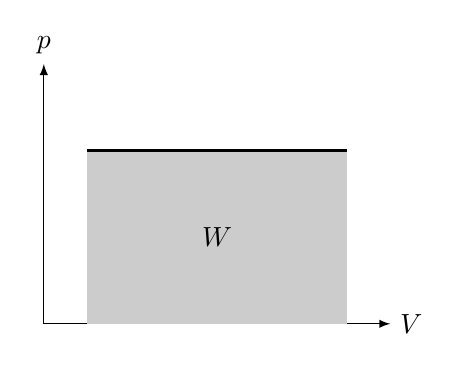
\begin{tikzpicture}[>=latex,scale=1.1]
   \draw[->] (0,0) -- (4,0) node[right] {$V$};
   \draw[->] (0,0) -- (0,3) node[above] {$p$};
 
   \fill[black!20] (0.5,0) rectangle (3.5,2);
 
   \draw[thick,black] (0.5,2) -- (3.5,2);
 
   \node at (2,1) {$W$};
 \end{tikzpicture}
\end{center}

\subsubsection{Transformaciones isotérmicas (temperatura constante)}

\[ pV = nRT = cte. \; \to p_1V_1 = p_2V_2 \quad \text{ó} \quad \frac{p_1}{p_2} = \frac{V_2}{V_1} \]

Dado que, en estas condiciones, $ p = \frac{n R T}{V} $

\[ W := \int_{V_1}^{V_2} F \cdot dx = \int_{V_1}^{V_2} pS \cdot dx = \int_{V_1}^{V_2} p\cdot dV = \int_{V_1}^{V_2} \frac{n R T}{V} \cdot dV = n R T \ln \frac{V_2}{V_1} \]

En cuanto a la gráfica $p$-$V$:

\begin{center}
  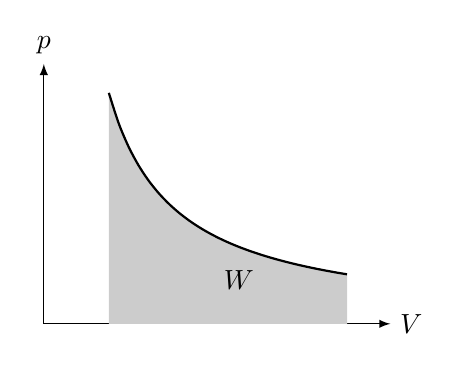
\begin{tikzpicture}[>=latex,scale=1.1]
    \draw[->] (0,0) -- (4,0) node[right] {$V$};
    \draw[->] (0,0) -- (0,3) node[above] {$p$};
    
    \fill[black!20,domain=0.75:3.5]
    (0.75,0)
    -- plot ({\x},{2/\x})
    -- (3.5,0)
    -- cycle;
    
    \draw[domain=0.75:3.5,smooth,variable=\x,thick,black]
    plot ({\x},{2/\x});
    
    \node at (2.25,0.5) {$W$};  
  \end{tikzpicture}
\end{center}

\subsubsection{Transformaciones isocóricas (volumen constante)}

\[ pV = nRT; \; \frac{V}{nR} = \frac{T}{p} = cte. \; \to \frac{T_1}{p_1} = \frac{T_2}{p_2} \]

Es fácil ver que $ W = 0 $ ya que $ \Delta V = 0 $.

\[ Q = n C_V \Delta T \to  (p_1 > p_2 \Leftto Q_1 > Q_2)\]

En cuanto a la gráfica $p$-$V$:

\begin{center}
\begin{tikzpicture}[>=latex,scale=1.1]
  \draw[->] (0,0) -- (4,0) node[right] {$V$};
  \draw[->] (0,0) -- (0,3) node[above] {$p$};

  \draw[thick,black] (2,0.5) -- (2,2.5);
  \node at (3,1.5) {$W=0$};
\end{tikzpicture}
\end{center}

\subsubsection{Transformaciones adiabáticas}

Sistemas perfectamente aislados o transformaciones instantáneas. Nada es constante.

\[ W = \frac{1}{1 - \gamma}(p_2V_2 - p_1V_1) \quad \text{donde } \gamma := \frac{C_p}{C_V} = \text{coef. adiabático} \]

Para el aire, $ \gamma \approx 1.4 $

En cuanto a la gráfica $p$-$V$:

\begin{center}
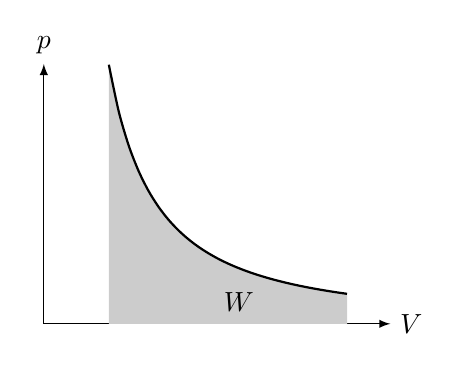
\begin{tikzpicture}[>=latex,scale=1.1]
  \draw[->] (0,0) -- (4,0) node[right] {$V$};
  \draw[->] (0,0) -- (0,3) node[above] {$p$};

  \fill[black!20,domain=0.75:3.5]
      (0.75,0)
      -- plot ({\x},{2/\x^1.4})
      -- (3.5,0)
      -- cycle;

  \draw[domain=0.75:3.5,smooth,variable=\x,thick,black]
      plot ({\x},{2/\x^1.4});

  \node at (2.25,0.25) {$W$};
\end{tikzpicture}
\end{center}

\subsection{Procesos reversibles e irreversibles}

Llamamos proceso reversible a aquel en el cuál en el proceso de transformación $ (p_0, V_0, T_0) \to (p, V, T) $ todos los estados intermedios son estables. Es decir, la transformación es lenta.

\subsubsection{Motores térmicos y máquinas frigoríficas}

Una máquina térmica basa su funcionamiento en el flujo de energía calorífica entre dos focos. Si saca calor de un foco caliente, lo vierte en otro frío, y aprovecha el trabajo resultante de la transformación, se llama \textbf{motor térmico}. Si por el otro lado saca calor de un foco frío utilizando trabajo y lo vierte en otro caliente, se llama \textbf{máquina frigorífica}.

En esta situación,

\[ W = Q_c - Q_f\]

\[ \eta := \frac{E_u}{E_a} = \frac{W}{Q_c} = 1 - \frac{Q_f}{Q_c} \]

\subsubsection{Ciclo ideal de Carnot}

Máximo rendimiento que se puede extraer de dos focos. El rendimiento es comúnmente aproximado tal que:

\[ \eta \approx 1 - \frac{T_f}{T_c} \]

Asumimos la transmisión calorífica perfecta en las expansiones y el aislamiento perfecto en las compresiones:

\begin{enumerate}
    \item \textbf{Expansión isotérmica}: Se aplica el calor del foco caliente, resultando en una expansión del gas a la misma temperatura que el foco caliente.
    \item \textbf{Expansión adiabática}: Se retira el foco caliente; el gas sigue expandiéndose debido a la energía cinética residual.
    \item \textbf{Compresión isotérmica}: Se aplica el calor del foco frío, retirando el calor del gas y dejándolo a la misma temperatura que la del foco frío.
    \item \textbf{Compresión adiabática}: Se retira el foco frío; el gas sigue comprimiéndose debido a la energía cinética residual.
\end{enumerate}

\begin{center}
\begin{tikzpicture}[>=latex,scale=1.1]
  \draw[->] (0,0) -- (4,0) node[right] {$V$};
  \draw[->] (0,0) -- (0,3) node[above] {$p$};

\end{tikzpicture}
\end{center}

\subsection{Motores de combustión interna}

Siempre nos vamos a encontrar con un pistón y una recámara. Por lo que distinguimos entre tipo de transformación que se produce en la aplicación del foco caliente, y número de movimientos del pistón (tiempos) en el que el ciclo se completa. 

\subsubsection{Motores de explosión}

Nos centramos en el ciclo de Otto.

\begin{itemize}
    \item \textbf{De 4 tiempos}: 
        \begin{center}
            \includegraphics[scale=0.5]{Ciclo_de_4_tiempos.JPG}
        \end{center}

        \begin{enumerate}
            \item \textbf{Fase de admisión}: transformación isobárica.
            \item \textbf{Fase de compresión}: transformación adiabática; transformación isocórica (explosión, combustión instantánea).
            \item \textbf{Fase de expansión}: transformación adiabática; transformación isopórica (apertura de la válvula).
            \item \textbf{Fase de escape}: transformación isobárica.
        \end{enumerate}
        
        \begin{center}
        \begin{tikzpicture}[>=latex,scale=1.1]
          \draw[->] (0,0) -- (4,0) node[right] {$V$};
          \draw[->] (0,0) -- (0,3) node[above] {$p$};
        
        \end{tikzpicture}
        \end{center}
   \item \textbf{De 2 tiempos}: 
        \begin{center}
            \includegraphics[scale=0.2]{Esquema-de-2-tiempos.jpg}
        \end{center}

        \begin{enumerate}
            \item \textbf{Fase de compresión y aspiración}: transformación adiabática; transformación isobárica.
            \item \textbf{Fase de explosión y escape}: transformación adiabática; transformación isobárica.
        \end{enumerate}
        
        \begin{center}
            \begin{tikzpicture}[>=latex,scale=1.1]
              \draw[->] (0,0) -- (4,0) node[right] {$V$};
              \draw[->] (0,0) -- (0,3) node[above] {$p$};
            \end{tikzpicture}
        \end{center}
\end{itemize}

\subsubsection{Motores de diesel}

Los motores diesel cambian la bujia que produce la explosión del combustible por un inyector (combustión progresiva).

\begin{itemize}
    \item \textbf{De 4 tiempos}:
        \begin{enumerate}
            \item \textbf{Fase de admisión}: transformación isobárica.
            \item \textbf{Fase de compresión}: transformación adiabática.
            \item \textbf{Fase de expansión}: transformación isobárica (combustión); transformación (adiabática).
            \item \textbf{Fase de escape}: transformación isocórica; transformación isobárica.
        \end{enumerate}
        \begin{center}
            \begin{tikzpicture}[>=latex,scale=1.1]
              \draw[->] (0,0) -- (4,0) node[right] {$V$};
              \draw[->] (0,0) -- (0,3) node[above] {$p$};
            \end{tikzpicture}
        \end{center}
    \item \textbf{De 2 tiempos}:
        \begin{enumerate}
            \item \textbf{Fase de compresión y aspiración}: transformación adiabática; transformación isocórica.
            \item \textbf{Fase de explosión y escape}: transformación adiabática; transformación isocórica.
        \end{enumerate}
        \begin{center}
            \begin{tikzpicture}[>=latex,scale=1.1]
              \draw[->] (0,0) -- (4,0) node[right] {$V$};
              \draw[->] (0,0) -- (0,3) node[above] {$p$};
            \end{tikzpicture}
        \end{center}
\end{itemize}

\subsubsection{Parámetros y magnitudes características}

\begin{itemize}
    \item \textbf{Calibre}: $ d := \text{diam.} $
    \item \textbf{PMS}: Punto muerto superior.
    \item \textbf{PMI}: Punto muerto inferior.
    \item \textbf{Carrera}: $ h := PMS - PMI$
    \item \textbf{Cilindrada}: $ V := \pi \frac{d^2}{4} h n \quad \text{donde } n := \text{núm. de cilindros} $
    \item \textbf{$V_c$}: Volumen cámara de compresión.
    \item \textbf{Relación de compresión}: $ RC := \frac{V_1 + V_c}{V_c} $
    \item \textbf{Gasto}: $ G := \frac{m_c}{t} $
    \item \textbf{Potencia absorbida}: $ P_a = G P_c \quad \text{donde } P_c = \text{poder calorífico} $
    \item \textbf{Momento de torsión}: $ M = F r $
    \item \textbf{Potencia útil}: $ P_u = M \omega $
\end{itemize}

\subsection{Motores de combustión externa}

Su utilidad es la generación eléctrica y de propulsor de aviones.

\subsubsection{Ciclo de Rankine (Turbina de vapor)}

\begin{center}
    \includegraphics[scale=0.3]{Ciclo_de_Rankine.jpg}
\end{center}

\begin{enumerate}
    \item \textbf{Caldera}: transformación isobárica: Absorción de calor en la caldera, comienza el cambio de fase, se produce vapor sobrecalentado.
    \item \textbf{Turbina}: transformación adiabática.
    \item \textbf{Condensación}: transformación isobárica; transformación isotérmica.
    \item \textbf{Bomba}: transformación isocórica.
\end{enumerate}

\begin{center}
    \begin{tikzpicture}[>=latex,scale=1.1]
      \draw[->] (0,0) -- (4,0) node[right] {$V$};
      \draw[->] (0,0) -- (0,3) node[above] {$p$};
    \end{tikzpicture}
\end{center}

\subsubsection{Ciclo de Brayton (Turbina de gas)}

\begin{center}
    \includegraphics[scale=0.5]{Ciclo_de_Brayton.png}
\end{center}

\begin{enumerate}
    \item \textbf{Compresor}: transformación adiabática.
    \item \textbf{Quemador}: transformación isobárica.
    \item \textbf{Turbina}: transformación adiabática.
\end{enumerate}

\begin{center}
    \begin{tikzpicture}[>=latex,scale=1.1]
      \draw[->] (0,0) -- (4,0) node[right] {$V$};
      \draw[->] (0,0) -- (0,3) node[above] {$p$};
    \end{tikzpicture}
\end{center}

\subsection{Bombas de calor}

La transmisión de calor de un foco frío a uno caliente no es espontánea. Por lo cual necesitamos realizar trabajo para que esto ocurra. Este trabajo será igual a la diferencia de calor de los
focos $ W = Q_C - Q_F $.

\subsubsection{Ciclo de refrigeración de Carnot}

Máxima eficiencia que se puede extraer de dos focos. El rendimiento es comúnmente aproximado tal que:

\[ \epsilon = \frac{E_u}{E_a} = \frac{Q_F}{W} = \frac{Q_C}{Q_C - Q_F} \approx \frac{T_C}{T_C - T_F} \]

Asumimos la transmisión calorífica perfecta en las expansiones y el aislamiento perfecto en las compresiones:

\begin{enumerate}
  \item \textbf{Compresión adiabática} Se realiza el trabajo comprimiendo el émbolo. Aumenta la temperatura y presión del gas.
  \item \textbf{Compresión isotérmica} Se aplica el foco caliente, que toma calor del gas.
  \item \textbf{Expansión isotérmica} Se retira el foco caliente, causando que el gas se expanda y disminuya su temperatura.
  \item \textbf{Compresión isotérmica} Se aplica el foco frío, que retira calor del gas.
\end{enumerate}

\begin{center}
    \begin{tikzpicture}[>=latex,scale=1.1]
      \draw[->] (0,0) -- (4,0) node[right] {$V$};
      \draw[->] (0,0) -- (0,3) node[above] {$p$};
    \end{tikzpicture}
\end{center}

\subsubsection{Ciclo de Rankine inverso}

\begin{enumerate}
  \item \textbf{Compresión adiabática}: El vapor saturado procedente del evaporador llega al compresor; aumenta su temperatura hasta alcanzar el punto
    correspondiente al vapor recalentado. Esta transformación se realiza con la aportación de trabajo externo ($ W $).
  \item \textbf{Transformación isobárica}: En el condensador, el vapor está a una temperatura mayor que la del ambiente, por tanto cede calor ($ Q_C $), manteniendo constante
    la presión, mientras se produce, primero, un enfriamiento seguido de una condensación hasta convertirse en líquido saturado. Al pasar de vapor a líquido hay una gran reducción
    de volumen, con lo cual el fluido pasa a un estado líquido a alta presión.
  \item \textbf{Expansión adiabática}: Se hace pasar el fluido por la válvula de expansión, donde se produce una transformación adiabática con un ligero aumento del volumen y
    gran disminución de presión y temperatura. Una parte del líquido se vaporiza, y en el punto 4 hay vapor húmedo.
  \item \textbf{Transformación isobárica} El vapor húmedo, a su paso por el evaporador, que se encuentra en el recinto que queremos refrigerar, absorbe calor del foco frío ($ Q_F $)
    por encontrarse a menor temperatura que éste. Se completa la vaporización del fluido a medida que aumenta su volumen hasta llegar a la entrada del compresor, donde comienza de
    nuevo el ciclo.
\end{enumerate}

Este ciclo puede servir tanto para refrescar en verano ($ Q_C = $ \textit{exterior}, $ Q_F =  $ \textit{interior}) como calentar en invierno ($ Q_C = $ \textit{interior},
$ Q_F =  $ \textit{exterior}). Asimismo tanto el evaporador como el condensador pueden intercambiar funciones. Concluimos que solo es necesario alternar el flujo del refrigerante
para alternar funciones.

\begin{center}
    \begin{tikzpicture}[>=latex,scale=1.1]
      \draw[->] (0,0) -- (4,0) node[right] {$V$};
      \draw[->] (0,0) -- (0,3) node[above] {$p$};
    \end{tikzpicture}
\end{center}

Cabe enumerar los distintos elementos presentes en la refrigeración por vapor. Estos son: compresor (puede ser centrífugo o volumétrico), condensador o evaporador (intercambiadores
de calor), válvula de expansión (mantiene la presión constante del refrigerante que se dirige hacia el evaporador).

\begin{center}
  \includegraphics[scale=0.5]{Ciclo_de_Rankine_inverso.png}
\end{center}

\section{Hidráulica y neumática}

\subsection{Elementos de los circuitos neumáticos}

Los circuitos neumáticos utilizan aire para su funcionamiento. Naturalmente, necesitaremos elementos que capten el aire, lo compriman, lo almacenen, regulen su presión, etc.
Por otra parte, elementos para dispensar del aire son innecesarios o muy simples.

\subsubsection{Compresores}

Encontramos dos tipos de compresores:

\begin{itemize}
  \item \textbf{Volumétricos}: Reducen el volumen que ocupa el aire, aumentando la presión, según la ley de Boyle. Podemos distinguir a su vez entre 
    alternativos o de pistón y rotativos.
  \item \textbf{Dinámicos}: Aumentan la energía cinética del aire que, al frenar contra el fluido ya existente en su salida hace que su velocidad se 
    transforme en presión de empuje según la ecuación de Bernoulli. Los tipos que existen son: radiales o centrífugos y axiales.
\end{itemize}

Los compresores suelen guardar el aire comprimido en un depósito.

\subsubsection{Acondicionadores del aire}

Con tal de no desgastar los elementos involucrados en el circuito, el aire pasa por un proceso de acondicionado:

\begin{enumerate}
  \item \textbf{Secador}: reduce el contenido de vapor de agua en el aire.
  \item \textbf{Filtro}: retiene las impurezas arrastradas por el aire.
  \item \textbf{Regulador de presión}: mantiene el valor de la presión constante.
  \item \textbf{Lubricador}: pulveriza una pequeña cantidad de aceite en el aire. Evita la corrosión y el desgaste interno
    de las piezas.
\end{enumerate}

La combinación de las tres últimas unidades dan lugar a la \textbf{unidad de mantenimiento}. Y la combinación de todos los
elementos, junto con el compresor, dan la \textbf{toma de aire a presión}.

\subsubsection{Actuadores neumáticos}

Diferenciamos entre actuadores rotativos (motores, usos escasos), y actuadores lineales (cilíndros). Nos centraremos en los lineales, los cuáles se subdividen en 2 tipos:

\begin{itemize}
  \item \textbf{De simple efecto}: El aire solo puede realizar una acción (típicamente la de extensión del pistón). El retorno se realiza por un muelle.
  \item \textbf{De doble efecto}: Tanto el avance como el retroceso viene dado por aire.
\end{itemize}

Nos suele interesar el cálculo de la fuerza y el consumo de aire.

La fuerza teórica viene dada por:

\[ F_t = p S \]

Donde $ S = S_e - S_v  $ en el retroceso de un pistón de doble efecto y $ S = S_e $ de lo contrario.

No obstante, uno debe tener en cuenta tanto la fuerza de rozamiento como el muelle, conque:

\[ F = F_t - F_r - F_m \]

Donde $ F_m = K \Delta x $. En otras ocasiones, $ F $ se toma de un porcentaje de $ F_t $.

El consumo de aire es precisamente el volumen de aire implicado en la acción del cilíndro, es decir, la carrera $ l $ por la superficie $ S $ (Con las consideraciones anteriores
de que es la superficie). 

\subsubsection{Válvulas distribuidoras}

Sirven para dirigir y regular la dirección del aire comprimido a través de los circuitos. Se nombran según el número de vías u orificios que tengan, el número de estados,
y su accionamiento.

\begin{center}
  \includegraphics[scale=0.8]{Tabla_Distribuidoras.jpg}
\end{center}

\subsubsection{Otras válvulas}

% poner imagenes

\begin{center}
  \begin{tabular}{| c | c | c |} 
    \hline
    Nombre & Uso & Imagen \\
    \hline
    Válvula antirretorno & Deja pasar el aire en un solo sentido & \includegraphics[scale=0.25]{Valvula_antirretorno.png} \\
    \hline
    Válvula reguladora bidireccional & Regula el caudal del aire & \includegraphics[scale=0.75]{Valvula_reguladora_bidireccional.png} \\
    \hline
    Válvula reguladora unidireccional & Regula el caudal del aire en un solo sentido & \includegraphics[scale=0.25]{Valvula_reguladora_unidireccional.jpg} \\
    \hline
    Válvula selectora de circuitos & Tiene una función lógica de OR & \includegraphics[scale=0.25]{Valvula_OR.png}\\
    \hline
    Válvula de simultaneidad & Tiene una función lógica de AND & \includegraphics[scale=0.25]{Valvula_AND.png} \\
    \hline
    Válvula temporizadora & Aplica un retardo en el pase del aire & \includegraphics[scale=0.25]{Valvula_temporizadora.jpg} \\
    \hline
  \end{tabular}
\end{center}

\subsection{Circuitos prácticos neumáticos}

\begin{itemize}
  \item \textbf{Mando de un cilindro de simple efecto con regulación de velocidad en el vástago}

\begin{center}
  \includegraphics[scale=0.5]{Mando1.jpg}
\end{center}

  \item \textbf{Mando condicional de simple efecto}

\begin{center}
  \includegraphics[scale=3.0]{Mando2.jpg}
\end{center}

  \item \textbf{Mando semiautomático de un cilindro de doble efecto}

\begin{center}
  \includegraphics[scale=0.5]{Mando3.png}
\end{center}

  \item \textbf{Mando automático de un cilindro de doble efecto}

\begin{center}
  \includegraphics[scale=0.5]{Mando4.png}
\end{center}
\end{itemize}

\subsection{Circuitos hidráulicos}

Son circuitos que emplean el aceite como fluido. Consecuentemente, podremos lograr mayor fuerza y sostener estados intermedios (fluido incompresible), 
tener mejor control caudal y velocidad, pero necesitaremos tuberías de recogida y habrá peligro de contaminación por fugas.

\subsubsection{Cálculo de parámetros en un circuito}

El principio de Pascal asevera que la presión ejercida sobre un fluido incompresible se transmite instantáneamente y por igual a todos los puntos de dicho fluido
($ p_1 = p_2 $ y $ V_1 = V_2 $). Por lo tanto, el caudal $ Q $ se mantiene a lo largo del circuito, conque la potencia hidráulica puede ser calculada tal que $ P = F v = p S v = p Q $.

Según la ley de la conservación de la energía, tenemos:

\[ E_P + E_C + E_{Pr} = E_P' + E_C' + E_{Pr}' \to mgh + \frac{1}{2}mv^2 + pS = mgh' + \frac{1}{2}mv'^2 + pS' \]

Conque, diviendo entre $ V $, llegamos a la ecuación de Bernoulli:

\[ \rho gh + \frac{1}{2} \rho v^2 + p = \rho gh' \frac{1}{2} \rho v'^2 + p' \]

\newpage

\part{Historia de la Filosofía}

\section{Preludio}

Los autores filosóficos pertinentes a la selectividad son: \textbf{Platón, Descartes, Nietzsche y Ortega} (si se elige el bloque
de problemas ontológicos y epistemológicos).

\subsection{Áreas de la filosofía}

Para todos los autores a presentar es ponderable leer sus obras cuando sea factible.

Antes de tratar la Historia de la Filosofía, es encomiable repasar los contenidos de esta. La filosofía ($ \phi \iota \lambda o \text{- ``amor'', } \sigma o \phi \iota \alpha \text{- ``sabiduría''} $)
es el estudio racional de los constituyentes fundamentales de la realidad y del ser humano. Es, en cierto sentido, el conjunto de axiomas que suponemos para el desarrollo de los demás conocimientos.

\subsubsection{Metafísica}

\subsubsection{Epistemología}

\subsubsection{Ética}

\subsubsection{Política}

\newpage

\section{Platón}

\begin{center}
  \includegraphics[scale=0.1]{platon.jpg}
\end{center}

\begin{center}
  \textit{Toda la filosofía occidental es una serie de notas a pie de página de Platón}
  
  Alfred North Whitehead
\end{center}

La influencia que ha tenido la filosofía de Platón sobre la filosofía y todas sus vertientes y todos los que beben de ellas, que en última
instancia es la humanidad completa, escapa de todo remarque. La posición maximalista de dicha proposición afirma que tras Platón,
\textit{nihil novum sub sole}.

Algunos Padres de la Iglesia miraron a Platón con gran veneración, y las sublimes verdades que se encierran en sus escritos y formaron tan
grandes filósofos, tuvieron bastante fuerza para arrancar de la docta pluma de San Agustín, hablando de éstos, aquella fuerte hipérbole: 
que en mudando algunas proposiciones y unos pocos términos se convertirían en hombres cristianos.

Cabe destacar que la distribución de contenidos de la presente exposición no sigue la del mismo Platón. No es hasta Aristóteles que se
conoce una manera sistemática de la presentación de la filosofía. Platón en particular presentaba sus obras en forma de diáogos (cuyo 
personaje principal suele ser Sócrates), que con libertad fluían entre distintos temas.

\subsection{Metafísica}

La filosofía platónica propone un esquema a aplicar en distintas áreas del saber, el llamado \textit{dualismo Platónico}, el cuál está expuesto 
con el símil de la caverna. La etimología de dualismo ya sugiere el fundamento que profesa, a saber: la existencia de dos principios fundamentales que
componen un sistema. El dualismo platónico además precisa la esencia de estos dos principios, o \textit{mundos} y la relación entre ellos. 

En metafísica, se postula un mundo sensible, inferior, el cuál es contingente, perecedero, imperfecto \dots (en definitiva, \textit{Hericlíteo}), que
se corresponde al mundo formal, superior, el cuál es inmutable, eterno, perfecto \dots (en definitiva, \textit{Parménico}), mediante participación e imitación.
Lo cuál quiere decir que el mundo sensible, compuesto de particulares, participa en sus correspondientes universales (exhibiendose como ejemplos del universal)
e imita la ideosincrasia de sus universales. Se deduce, además, que ambos mundos son independientes y, en cierto sentido, el mundo formal es anterior.

La aplicación del dualismo platónico a la metafísica resulta en la llamada \textit{Teoría de las ideas}, que es la previamente expuesta. Es por su primacía en
las ideas que esta teoría constituye la primera filosofía idealista en la Historia de la Filosofía.

A este nivel cabe destacar además la existencia de una Idea suprema: el Bien. Para Platón esta es la Idea que da sentido al resto. En el simil de la caverna
el Bien se identifica con el sol puesto que proporciona la luz por la que podemos dislumbrar el resto de Formas. Resulta esto importante ya que en la genealogía
de Dios dicha concepción es primordial. En este símil también cabe la explicación de una característica crucial de esta concepción de Bien. A saber, Platón concibe
de un Bien que es inefable, el cuál es exclusivo a la revelación mística.

\subsubsection{Ontología}

En misma correspondencia con los anteriores mundos, encontramos dos tipos de cosas que ``son'': Lo \textit{particular} y lo \textit{universal}. Platón distingue al
menos en 4 maneras entre estas dos categorías, a saber: multiplicidad, siendo lo universal único y lo particular múltiple, tal que un único fenómeno pueda presentar
distintos ejemplos; mutabilidad, puesto que lo universal es rígido e inmóvil mientras que lo particular es contingente; materialidad, de manera que las Formas
transcienden cualquier marco material, opuestamente a la manera en la que lo particular se encuentra ligado a la materia; sensibilidad, tal que el órgano que percibe
las Ideas es la mente, el \textit{alma}, y el que percibe los particulares son los sentidos.

De esta manera, la perfección es una cualidad exclusiva a los universales, puesto que el ejemplo siempre carece de algo respecto a su Idea (cf. ejemplo del triángulo).

% \subsubsection{Cosmología} (Demiurgo)

\subsection{Epistemología}

Platón distingue rigurosamente entre lo que puede ser objeto de conocimiento auténtico (\textit{epistéme}) y lo que pertenece al campo de la opinión (\textit{doxa}). 
El conocimiento verdadero no trata de particulares sensibles, cambiantes y engañosos, sino de las Formas o Ideas, entidades inmutables y universales que constituyen la
realidad ontológicamente prioritaria. Así, epistemológicamente, conocer equivale a participar intelectualmente en la Forma correspondiente: no basta la percepción sensorial
para aprehender la esencia de las cosas.

Dos figuras explicitan este pensamiento: el mito de la caverna y la \textit{línea dividida}. En la línea dividida Platón traza, de menor a mayor grado de verdad, los segmentos de
la imaginación y la creencia (los cuales remiten al mundo sensible), y los de la comprensión matemática y la dialéctica (propios del mundo inteligible). La dialéctica, entendida 
como arte del diálogo y de la refutación sistemática, culmina en la intuición racional de las Formas y, sobre todo, en la contemplación del Bien, que ilumina y legitima todo saber: 
conocer el Bien es, en última instancia, conocer la condición de posibilidad de la verdad.

\begin{center}
  \includegraphics[scale=0.5]{Simil_de_la_linea.png}
\end{center}

Otra tesis epistemológica central es la Teoría de la reminiscencia o \textit{anamnésis}: el alma, al ser inmortal y haber contemplado las Formas antes de su encarnación, 
recuerda mediante la correcta interrogación y el ejercicio intelectual lo que ya en ella existe latente. La educación, por tanto, no es mera transmisión de información sino 
recolocación (o evocación) de la verdad que el alma ya posee; la mayéutica socrática es la técnica educativa que facilita esa recolección de la verdad mediante preguntas dirigidas.

Platón jerarquiza también las disciplinas: las matemáticas ocupan un lugar preparatorio, pues habituan la mente a la abstracción, mientras que la dialéctica constituye 
la forma suprema de conocimiento, puesto que por ella se trasciende el plano hipotético y se alcanza el conocimiento de los principios primeros.

\subsection{Antropología}

La tan reconocida distincción entre cuerpo y mente (\textit{alma}) proviene al instanciar el dualismo platónico al humano. Siendo el alma
el mundo superior, se deriva: la imperativa al asceticismo, que el cuerpo sirve como prisión para el alma, el ciclo de reencarnación 
(metensicosis) \dots . Es aquí donde es posible trazar una influencia hacia los Pitagóricos y a su vez hacia el orfismo.

\subsubsection{Alma}

El alma, según Platón, tiene carácter divino y es ontológicamente prioritaria respecto del cuerpo. Es inmortal, preexistente y capaz de contemplar las Formas; 
su caída al cuerpo es lo que origina el olvido y la necesidad de aprendizaje que, en realidad, es recolocación. Moralmente, el alma es tripartita, conforme a la 
célebre división de \emph{La República}:

\begin{itemize}
  \item \textbf{La parte racional} (\textit{logistikon}): orientada al conocimiento, ama la verdad y debe gobernar por su capacidad para discernir el Bien.
  \item \textbf{La parte irascible o espirituosa} (\textit{thymoeides}): vinculada al ánimo, al honor y al valor; su función es auxiliar a la razón y sostener la firmeza moral. 
  \item \textbf{La parte concupiscible} (\textit{epithymetikon}): relacionada con apetitos y placeres corporales; exige moderación.
\end{itemize}

Platón relaciona la anterior división con las 4 virtudes griegas \textit{cardinales} (a saber: prudencia, justicia, coraje y templanza) de la siguiente manera:

\begin{itemize}
  \item Que haya \textbf{prudencia} significa que la parte racional sea la autoridad suprema y guie al resto.
  \item Que haya \textbf{coraje} significa que la parte irascible se someta la parte racional. Puesto que son valientes aquellos que, sabiendo lo que es bueno, actuan
        de manera acorde.
  \item Que haya \textbf{templanza} significa que la parte concupiscible sepa moderar su apetito, así subordinandose a la razón.
\end{itemize}

Por último, la justicia, en el alma, se define como la armonía y el correcto ordenamiento entre estas partes: cada una desempeña su función sin usurpar la propia de las otras, bajo la dirección 
de la razón. En el plano antropológico-religioso, Platón postula el ciclo de transmigraciones y la posibilidad de purificación moral del alma (cf. el mito de Er), donde la conducta 
en la vida determina su suerte posterior.

\subsubsection{Cuerpo}

Siendo el cuerpo la antítesis del alma, Platón lo presenta como principio mortal, ligado a la generación y la corrupción, y como fuente de pasiones, deseos y errores perceptivos. 
Los sentidos remiten al mundo cambiante y, por tanto, son instrumentos limitados y frecuentemente engañosos para acceder a la verdad. La presencia del cuerpo impone sobre el alma 
tentaciones que desordenan su jerarquía, la concupiscencia puede subyugar a la razón si no mediatiza la educación y la disciplina moral; por eso Platón adopta, en sus consecuencias 
prácticas, una inclinación hacia el ascetismo moderado y la purificación.

No obstante, Platón no reduce el cuerpo a mero estorbo: reconoce su papel en la acción política y social y en la formación del carácter. El proyecto educativo que propone orienta y 
regula los impulsos corporales mediante gimnasia, música y disciplina, integrándolos de modo que sirvan a la excelencia del alma. La medicina del alma, como metáfora, exige ordenar 
y domesticar las apetencias para que la polis y la vida individual alcancen la armonía justa.

\subsection{Política}

La misión última de la filosofía política de Platón es la justicia. Su más magna obra expuesta para este fin es \textit{La República}.

Justicia se ha de entender por este nombre lo que en común llamamos virtud, y de otro modo hombría de bien, o concierto y armonía universal
de las acciones; es decir, aquel hábito de vivir en un todo conforme al dictamen de la recta razón que constituye al que le posee en la 
clase de hombre justo. Tomada la justicia en este sentido generalísimo, se identifica con la república concertada y estrechamente unida, de
forma que parezca no más de una sola alma; y la verdadera república equivale a la justicia de todos los ciudadanos , por la cual cada uno 
desempeña su cargo u oficio como es debido. En algo, no obstante, pueden distinguirse, e cuanto a la república es como el argumento y 
manteria de que se vale, y la justicia es como el fin y término; de modo que Platón toma por objeto una república, con el fin de manifestar
en rande, en términos que a nadie se le oculte, la naturaleza de la justicia.

Cinco puntos insinúa Platón en la introducción de su diálogo, que son como otras tantas piedras fundamentales sobre que se sustenta una
república; a saber: las solemnidades sagradas, la amistad, la prudencia y consejo de los ancianos, el afecto moderado de las riquezas, y
la utilidad de ellas para sostener los derechos de la verdad, compañera inseparable de la justicia.
\sn{
  En este primer punto, con la oración y la adoración, sacrificios y votos de los asistentes a las solemnidades sagradas, se indican la
  piedad y religión dos frmes fundamentos del Estado y de la justicia y demás virtudes necesarias a la sociedad; añadiendose a estos como
  terero la esperanza de los premios y temor de las penas que acaso es el más poderoso de los tres para contener la multitud.
}

La estructura política ideal platónica deriva directamente de la antropología tripartita: la ciudad perfecta replica en lo social el orden del alma justa. 
Así se distinguen tres clases sociales análogas a las partes del alma:

\begin{itemize}
  \item \textbf{Gobernantes (filósofos–reyes)}: corresponden a la parte racional. Solo aquellos que han alcanzado la comprensión de las Formas, y en última 
    instancia del Bien, son aptos para gobernar. La filosofía, convertida en virtud política, legitima el poder.
  \item \textbf{Auxiliares (guardianes guerreros)}: corresponden a la parte irascible. Su función es defender la ciudad y aplicar las decisiones de los gobernantes; 
    deben poseer coraje y lealtad.
  \item \textbf{Proveedores o productores (agricultores, artesanos, comerciantes)}: corresponden a la parte concupiscible. Su tarea es sostener materialmente la 
    polis mediante el trabajo y la producción.
\end{itemize}

La justicia política, por tanto, consiste en que cada clase realice la función para la cual está naturalmente más capacitada, bajo la guía de la razón gobernante. 
Para asegurar este orden, Platón propone medidas educativas y institucionales singulares: una educación pública y estricta para los guardianes, la formación filosófica 
progresiva de los futuros gobernantes, la supresión de la propiedad privada y de la familia entre los guardianes (con el fin de evitar intereses particulares), y la censura 
rigurosa de la poesía y los mitos que puedan corromper las costumbres. Es notorio el recurso del llamado \emph{mito de las clases} o \emph{mito de las raíces de metales} 
(el “noble engaño”), mediante el cual se mantiene la cohesión social y la aceptación del orden.

También es relevante la defensa platónica de la igualdad de capacidades: las mujeres aptas para el papel de guardián han de recibir la misma educación que los hombres en la 
ciudad ideal, quedando subordinada la selección al mérito y no al sexo.

Platón analiza asimismo la dinámica de degeneración política: la ciudad ideal puede decaer en distintos regímenes (timocracia, oligarquía, democracia) hasta culminar en la tiranía, 
cada uno con su psicología moral y sus vicios correspondientes. La causa última de este declive es el desorden interior del alma colectiva: cuando la razón deja de mandar, los apetitos 
y los intereses particulares toman el poder, provocando corrupción y violencia.

Finalmente, la figura del filósofo-rey sintetiza la aspiración platónica: un gobernante que no busca el poder por interés personal sino por saber y por amor a la verdad, capaz de 
orientar la polis hacia el bien común. La política platónica, aunque aristocrática en su designio (gobierno de los mejores en conocimiento), está animada por la idea de que el saber 
auténtico es condición de la legitimidad y la virtud públicas.

\newpage

\part{Lengua}

\section{Preludio}

\newpage

\end{document}
